\chapter{Preparation}\label{ch:prep}

The project builds upon an existing foundation of tools and concepts.
This chapter introduces the Elixir language used in its implementation, as well as providing a brief summary of concepts already described in the original Dataflow paper.
The professional Software Engineering approach used throughout is also touched upon.

\section{The Elixir programming language (a primer)}\label{sec:prep:elixir}

Elixir is a modern, functional language which executes on the BEAM VM, the standard VM used by Erlang.
This section provides only a short description of the language to give context for the implementation chapter.
Any special syntax or semantics in code examples will be explained where introduced.

\subsection{Language basics}

Elixir is a dynamically-typed, garbage collected functional language.
Values are immutable and looping behaviours are implemented through recursion, making use of tail-call optimisation, as in many other functional languages.

Elixir has the usual assortment of useful data types including arbitrary-sized integers, arbitrary-sized tuples, lists, maps (dictionaries) and binaries (which specialise to strings).

It also has the concept of \emph{atoms}, denoted \exs{:foo}.
Atoms are constant literals, with their name as their value, and can be compared very efficiently.

As such, atoms are used very often to tag tuples, for example \exs{{:ok, result}}.
These tagged tuples are very flexible and often replace the role that abstract data types in more classical functional languages.

Elixir has first-class functions and supports both defining lambdas and capturing existing functions within modules as lambdas.
All values in Elixir can be serialised in a standard way.
This includes functions and modules, which are serialised in their bytecode form.
That property makes it very easy to ship code over the wire, facilitating the distribution of work across a system.

Elixir also has powerful pattern-matching capabilities, available in function heads and \exs{case} expressions.
Since all values in the language can be directly expressed in the syntax (there are no user-definable types) any value can be directly matched, and values such as tuples, maps and lists can be destructured and their contents matched directly.
An example of combining pattern matching and atoms can be seen in \cref{lst:prep:pattern-matching-example}.

\begin{listing}[h]
	\caption{An example of using pattern-matching alongside tuples tagged with atoms.}
	\label{lst:prep:pattern-matching-example}
	\begin{minted}{elixir}
@doc """
Takes a widget, or a list of widgets, and returns its name
(in the case of a list the name of the first widget is returned).

Raises an error if the operation fails. 
"""

# This version of the function is only executed
# when the argument is a list with at least one element.
def get_widget_name!([widget | _]) do
  get_widget_name(widget)
end

# Maps are denoted %{}.
# %Widget{} is a special type of map, with an associated module.
# It is called a structure.
def get_widget_name!(%Widget{id: widget_id}) do
  case WidgetManager.get_name(widget_id) do
    {:ok, name} -> name
    {:error, reason} -> raise reason
  end
end

# If the function is called with an argument that is neither a list
# nor a %Widget{}, a runtime match error is raised.
	\end{minted}
\end{listing}


Elixir uses modules to organise functions.
A module is simply a namespace in which functions and macros, both public and private, can be placed.
Module names are atoms themselves, and in fact we can store them pass them around, dynamically calling functions within them at runtime.

Elixir has a very powerful macro system, which allows for the arbitrary transformation of the AST at compile-time.
In fact, most of the standard language directives such as those which define modules and functions or control the flow of the program are themselves macros.

Elixir programs often adopt the paradigm of data being transformed by flowing through a pipeline of functions.
To that end, the convention in Elixir for functions which operate on data is to take the thing being transformed as the first argument to the function.
Then, we make use of the pipeline operator \exs{|>} to write things like
\begin{minted}[linenos=false]{elixir}
"foo"
|> String.capitalize()
|> String.pad_leading(5)
# produces "  FOO"
\end{minted}
which is equivalent to
\begin{minted}[linenos=false]{elixir}
String.pad_leading(String.capitalize("foo"), 10)		
\end{minted}
but expresses the steps in the computation much more clearly.
This convention matches the Dataflow Model well, since it too works in terms of defining a pipeline of transformations for data to flow through.

\subsection{Concurrency model and the OTP framework}

Elixir and Erlang have a concept of processes, which are very lightweight userspace threads managed by the VM itself and scheduled transparently across hardware threads.
The VM can support many thousands (sometimes millions) of processes with a predictable, linear performance curve (rather than suddenly ``falling off a cliff'' under load), making it very suitable for writing highly concurrent systems.
Processes each have their own heap and can communicate and synchronise through a message-passing paradigm.
Data passed in a message is copied.

The OTP\footnotemark\ Framework ships with the standard Erlang distribution and provides a way to develop robust concurrent and distributed systems, affording powerful tools to isolate, monitor and act on failures.
It is used to organise processes into supervision trees, with certain processes responsible for starting, supervising (monitoring for crashes and errors, and potentially restarting) as well as killing child processes.
In this way we can isolate failures and handle them explicitly, giving the programmer the tools to create robust and failure-tolerant systems.

\footnotetext {
Once ``Open Telecom Platform'', the initialism now has no further meaning.
}

OTP also provides powerful concurrency primitives such as state machines and generic servers which handle many common edge cases and failure modes so prevalent in distributed systems.
It also allows for the connection of multiple BEAM nodes into a cluster, allowing for the transparent sending of messages between processes on different nodes.

It is a typical pattern to use these primitives to build systems with an actor model---isolated processes each handling a particular concern, communicating by sending messages.

While only a small portion of the power of OTP is used in the implementation in this project, a full production-ready distributed implementation of the Model in Elixir would be able to take advantage of the many advanced primitives available, greatly reducing code complexity and potentially increasing performance when compared to the JVM implementations.
In fact, many thousands of lines of code in the Java implementation are dedicated to solving the same problems and implementing the same features that one gets ``for free'' by using the BEAM VM.

\section{The Dataflow Model explained}\label{sec:prep:dataflow}

As mentioned in \cref{sec:intro:motivation}, the main feature of the Dataflow model is flexibility.
It aims to create a unified model of data processing which can encompass other processes, placing them in a well-defined structure and allowing the efficient execution of such systems.

It does this by separating the logical notion of data processing from the underlying physical implementation.
An abstract data processing model is defined which covers existing modes of processing by allowing the orthogonal specification of \textbf{what} results are computed, \textbf{where} in event time they are computed, \textbf{when} in processing time they are materialised, and \textbf{how} earlier results relate to later refinements \cite[p.~1793]{Akidau:2015}.

This standard model can then be implemented and realised by many different \emph{runners}, whether natively batch, streaming or hybrid, each with its own set of advantages and disadvantages. 
This flexible approach allows for the tuning of execution technology to business requirements while working with a consistent, expressive theoretical model of the processing itself.

The key takeaway is that this model tries to make as few assumptions as possible on the data inputs, outputs and processes, instead providing simple primitives from which complex system can be constructed.

What follows is a descriptions of the primitive concepts used in the model to more precisely specify all of these properties.

\subsection{``The What'': Transforms and pipelines}\label{sec:prep:dataflow:what}

In the Dataflow model, a \emph{pipeline} is an entire data processing flow.
It may incorporate many different \emph{transforms} which pass data between each other, processing and transforming it as it flows through them.
One can think of pipelines as Directed Acyclic Graphs (DAGs), with nodes representing transforms and edges representing the data flowing between them.

\begin{figure}[t]
	\subfloat[][A simple Pipeline which reads elements, counts the number of values for each key, and saves this result to a file.]{
	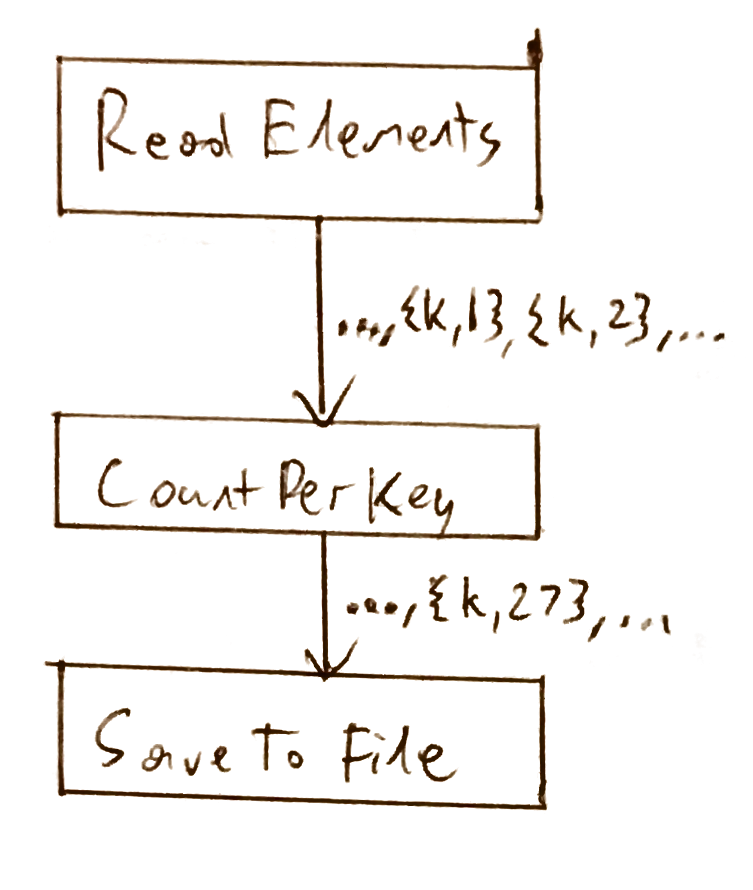
\includegraphics[width=0.3\textwidth]{images/temp/pipeline-dag-basic}
	}
	\subfloat[][A complex Pipeline featuring branching and Transforms with multiple inputs and outputs. Posts are read from a stream, and partitioned into important and regular posts based on a live stream of users currently considered important. \par Regular posts are mined for hashtags and a top-list of those is published to a Kafka topic. Important posts are processed to extract any brand mentions, and the top 50 brands for a particular window of time are extracted. These are merged with the top hashtags from ``regular'' posts, and the top-list emailed to select subscribers and saved off to cloud storage.]{
	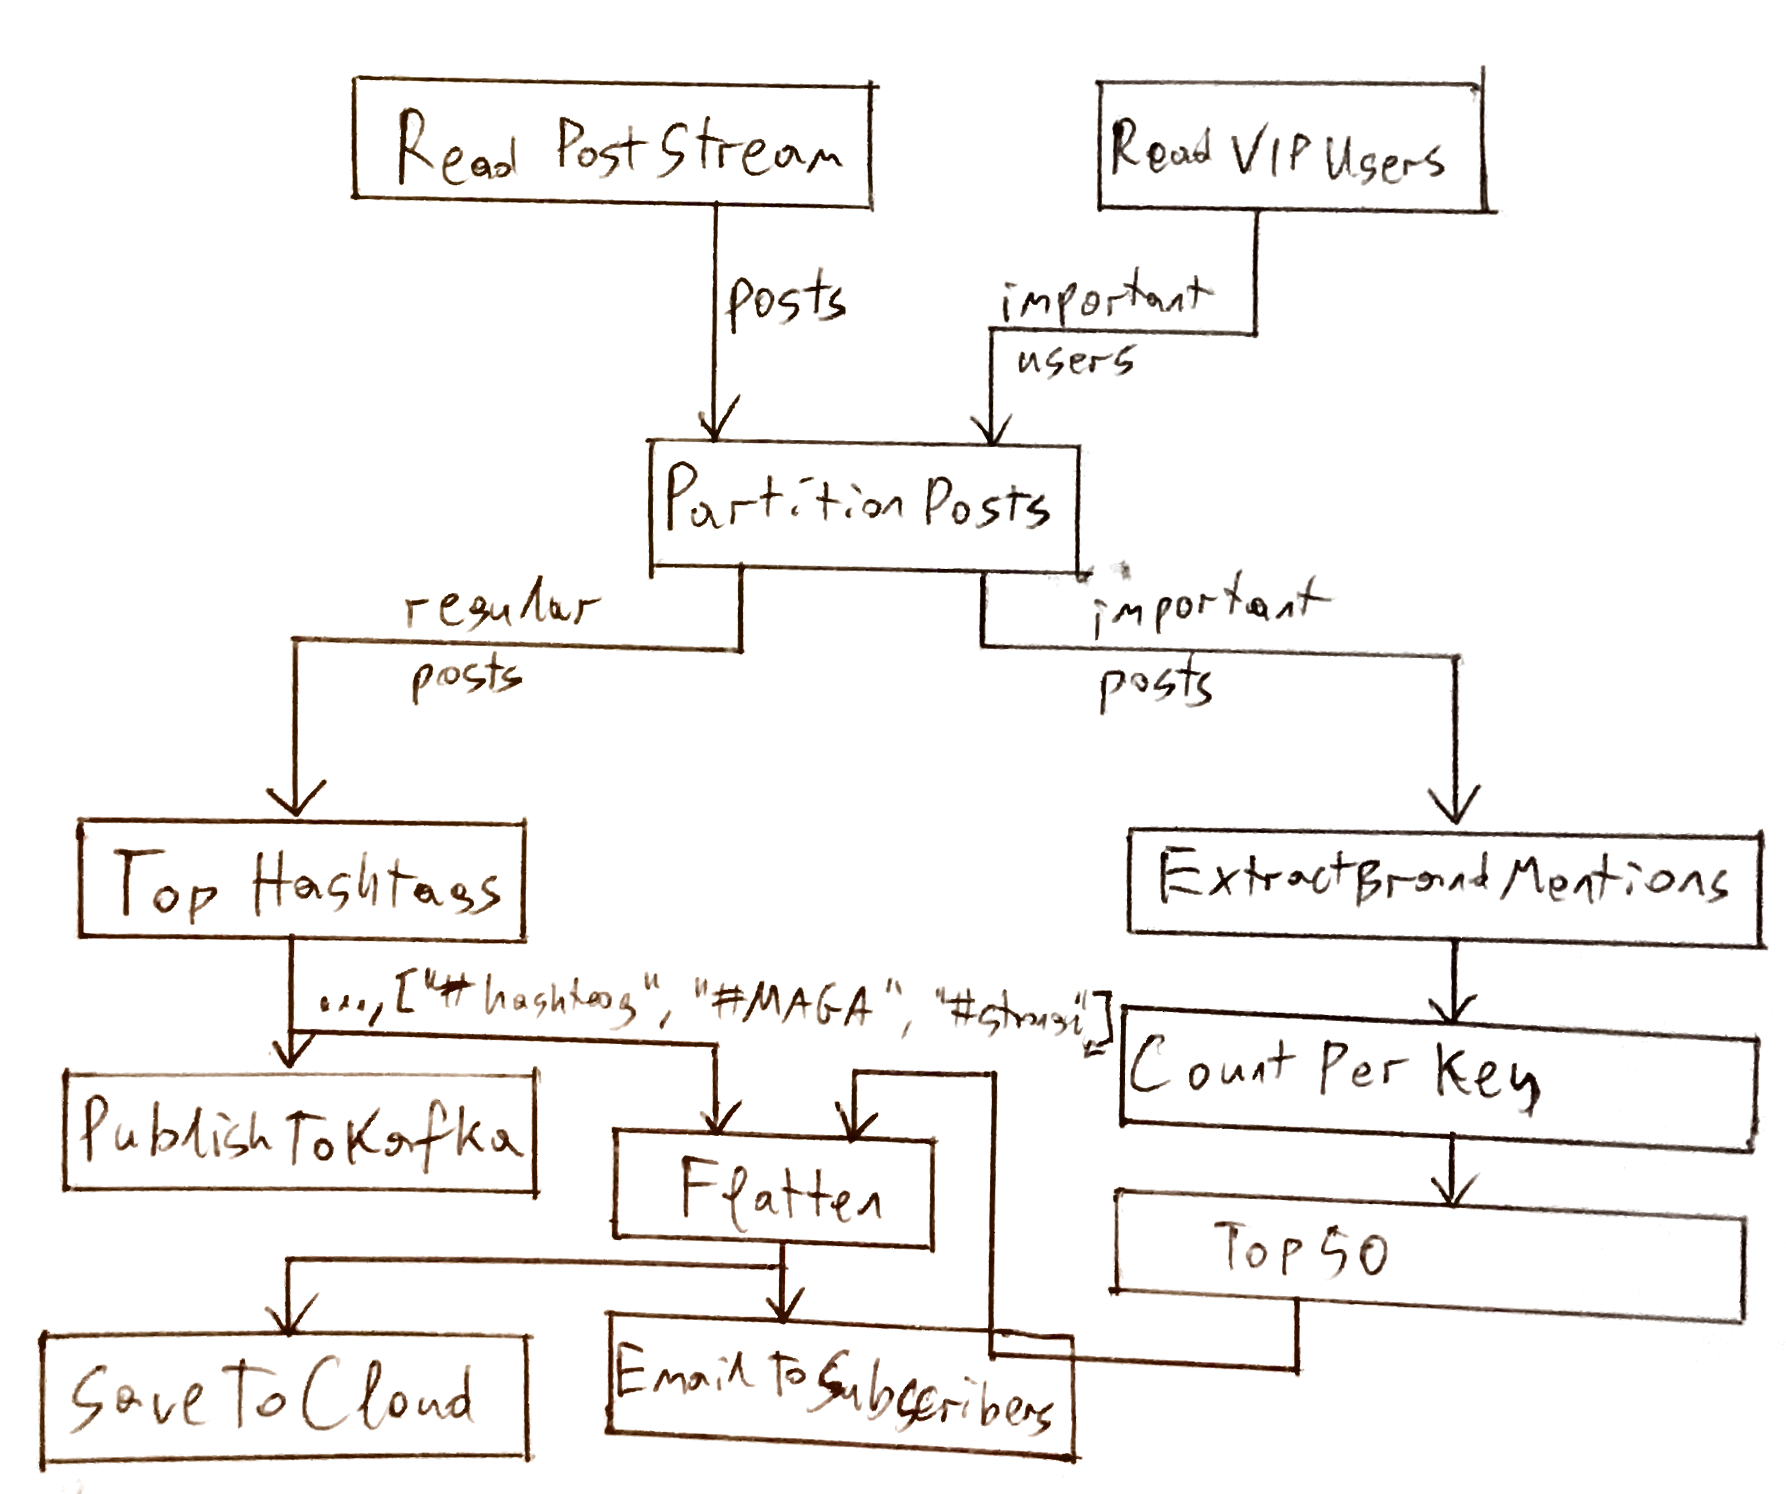
\includegraphics[width=0.7\textwidth]{images/temp/pipeline-dag-complex}
	}
	\caption{Examples of Pipelines, simple and complex, illustrated as DAGs.}
	\label{fig:prep:pipeline-dags}
\end{figure}

The graph does not have to be connected---it is valid for there to be multiple disjoint data processing paths.
A given transform may produce multiple outputs and it may take in multiple inputs.
It can also produce no outputs, instead causing a side effect such as writing to the network, database or file system.
Transforms can also have no inputs in the graph, instead receiving output from an external source or generating it.
These transforms are called root transforms.

A key advantage of expressing transforms in terms of data flowing is the natural adaptation of the system to unbounded data.
When we say unbounded data, we mean data which may not necessarily have an end.
An example of this may be a stream of events from a website, or the Twitter firehose.
It may help to think of unbounded data as ``streaming'' data, but ``streaming'' and ''batch'' imply execution strategies as opposed to data properties.
Further, in the Dataflow Model it is more convenient to think of all data as streamed, whether they form a true infinite stream, or are merely being streamed from a file or other bounded source.

It is worth making the distinction between building the pipeline by conceptually ``connecting'' the different transforms, and actually executing the pipeline with real data.
In the first case, what we are producing is a description of the running pipeline---we describe what the transforms should do, and what the data flowing between them will look like.
When we execute the pipeline, we need to materialise the transforms as some sort of structure which executes the processing steps declared earlier.
The data flowing through at execution-time is made up of elements which can be thought of as tuples with the data itself (often assumed to be key-value pairs), timestamps (intrinsic to the element) and any windows which have been assigned to the element (described later).

All transforms can be represented fundamentally using only two primitives: \verb|ParDo| and \verb|GroupByKey|\footnotemark[2].

\footnotetext[2]{
Even though these transforms are the only primitives mentioned in the original description of the Model \cite[§2.1]{Akidau:2015}, real implementation will likely special-case several other transforms such as \texttt{AssignTimestamps} or \texttt{Window} and make them primitives for architectural or performance reasons.
}

\begin{figure}[h]
	\centering
	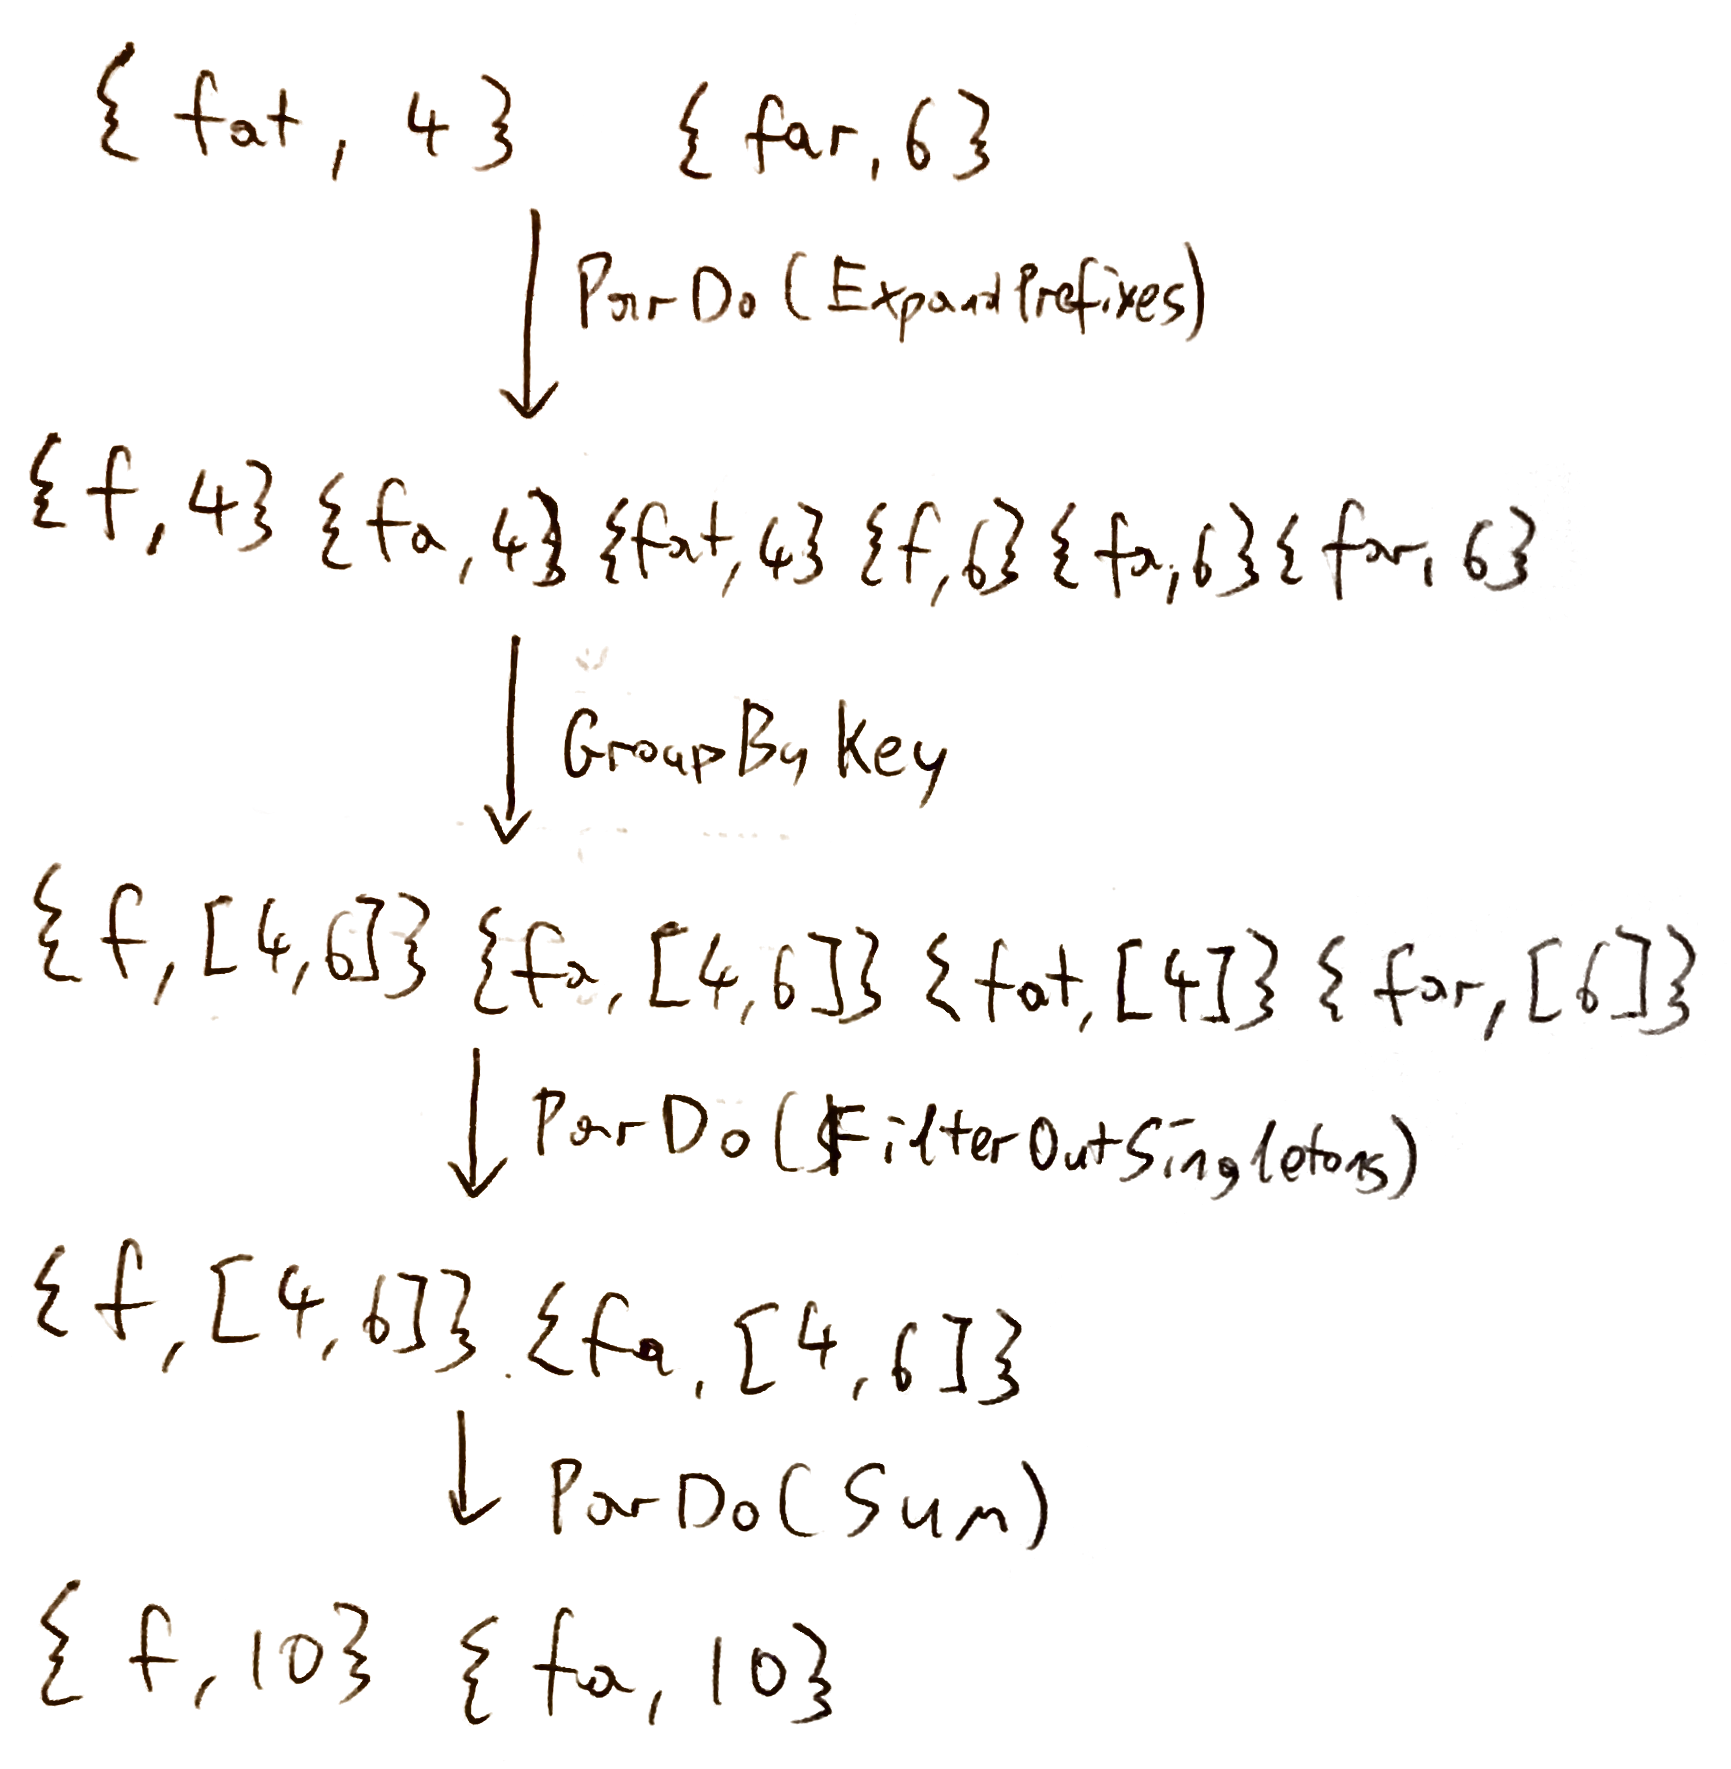
\includegraphics[width=0.6\textwidth]{images/temp/pardo-gbk}
	\label{fig:prep:pardo-gbk}
	\caption{An illustration of the operation of \texttt{ParDo} and \texttt{GroupByKey}. \texttt{ParDo} outputs zero or more elements per element, and \texttt{GroupByKey} outputs precisely one element per key in the input collection.}
\end{figure}


\verb|ParDo| represents a flat-map operation---it transforms an input data element into zero or more output data elements.
The actual computation performed can be arbitrary---the only restriction is that the output depends only on the single input element.
This restriction means that the \verb|ParDo| step is embarrassingly parallelisable (with caveats, as always).
It also translates naturally to operating on unbounded data, as we can emit the output in real-time.

\verb|GroupByKey|, on the other hand, simply groups all key-value pairs into elements with a single key and a collection of elements.
It needs to collect \emph{all} of the data for a particular key before being able to emit its output.
An issue arises when dealing with unbounded data---how do we know when we've received all of the input for a particular key?

To deal with this problem, the Dataflow Model introduces a concept of windowing.

\subsection{``The Where'': Windowing}\label{sec:prep:dataflow:where}

Windowing simply means the additional grouping of elements according to their timestamps in a way which allows us to emit a particular chunk of elements when we know that we have all the data for it.
In the Dataflow Model, we call such a chunk of data belonging to a particular window a \emph{pane}.
Before diving into the details, let us take a brief detour into what ``time'' means in this context.

\subsubsection{Time domains}
We distinguish between two inherent time domains when considering our data as events in time: \emph{event time} and \emph{processing time}.

Event time is the time at which the event actually occurred and is an inherent property of the element itself.
We also refer to this value as the \emph{timestamp} of an element.
Each element in a pipeline must have a timestamp.
We ensure that we have two ``special'' values available, the \emph{minimal} and \emph{maximal timestamps}.
Implementations may make these actual special values, or just use the maximal and minimal values of the underlying representation.

Where there is no inherent time associated with an element (for example it is an un-dated record in a file) or we don't know the timestamp yet (we must process the record before we can extract the timestamp), the element is assigned the minimum timestamp.
The logic of this will become apparent in the following sections.

Processing time is the property of an executing pipeline.
It measures real-world time elapsing as the computation progresses.
The processing time of a particular element at a particular transform is simply the system clock time at which it was seen or processed by that transform.
The Model makes no assumptions about the synchronisation of this time across multiple distributed transforms.

\subsubsection{Types of windows}

\begin{figure}[t]
	\subfloat[][Global window]{
		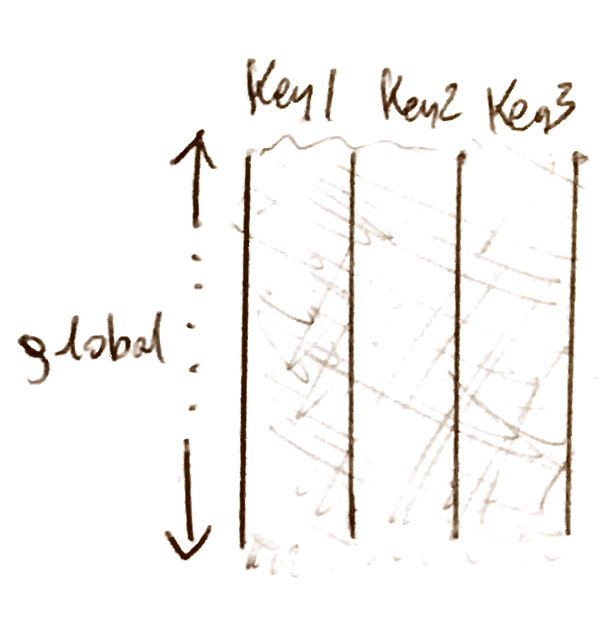
\includegraphics[width=0.25\textwidth]{images/temp/window-type-global}
	}
	\subfloat[][Fixed windows]{
		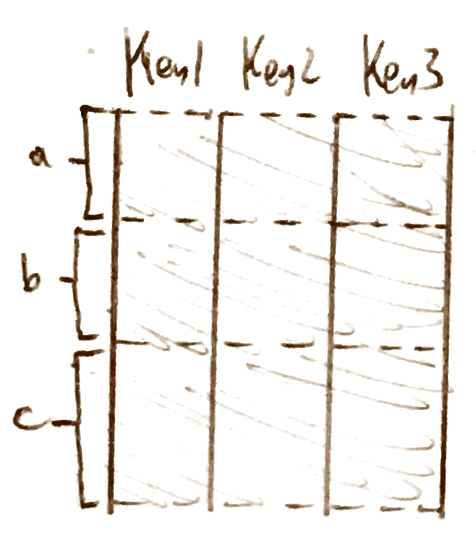
\includegraphics[width=0.25\textwidth]{images/temp/window-type-fixed}
	}
	\subfloat[][Sliding windows]{
		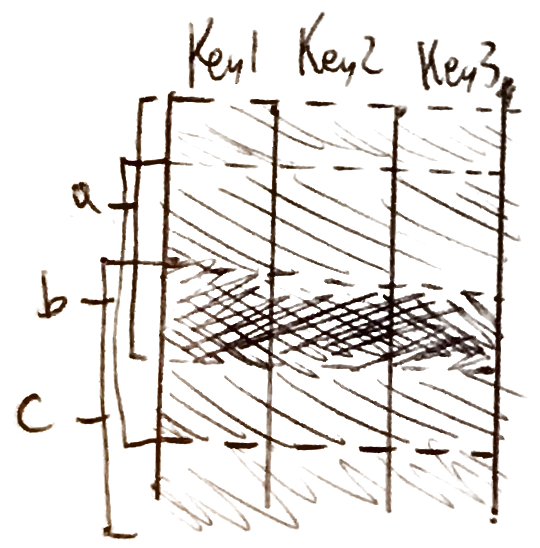
\includegraphics[width=0.25\textwidth]{images/temp/window-type-sliding}
	}
	\subfloat[][Sessions]{
		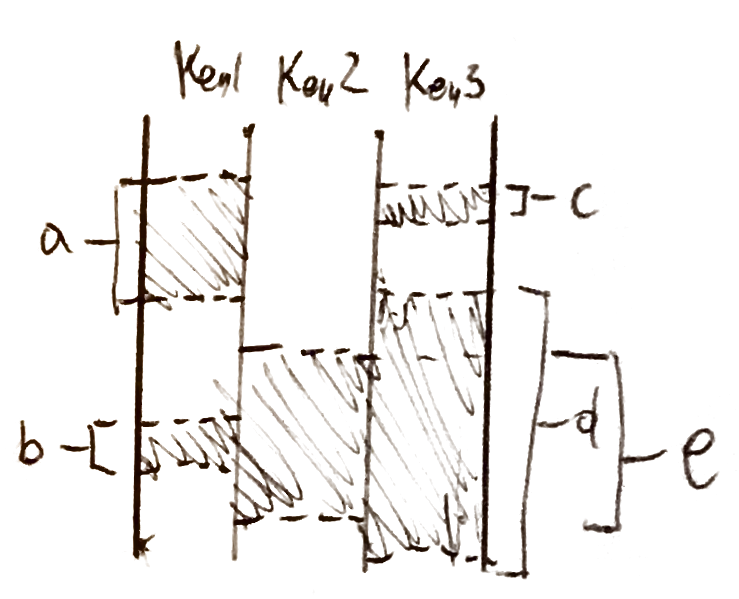
\includegraphics[width=0.25\textwidth]{images/temp/window-type-sessions}
	}
	\caption{Four windowing paradigms, all supported by the Dataflow Model.}
	\label{fig:prep:window-types}
\end{figure}

There are three windowing patterns which are most commonly used in practice.
\Cref{fig:prep:window-types} illustrates these, along with global windowing.

Global windowing simply assigns all elements to a single, infinitely large window.
It is the same in behaviour as having no windowing at all, but in the Model we still explicitly treat the global window as any other.

Fixed windows have a static window size, e.g.\ hourly, and are \emph{aligned}---each window contains all of the data in the system for that period of time.
Many data processing systems support this type of windowing.

Sliding windows have a static window size and slide period, e.g.\ hourly windows which start every 10 minutes.
In general, the windows may overlap, which requires the system to be able to place a single piece of data in multiple windows.
The windows are still aligned, meaning that each window applies across all of the data.

Sessions are windows which capture some period of activity over a subset of the data.
They are typically specified using a timeout after which a new session starts.
Any events closer in time than that form a session.
These windows need to be able to merge as new data is added between them.
They are also unaligned---certain windows apply only to a subset of the data.

These increasingly complex window types show a progression in complexity.
The Dataflow Model is able to support all of these by not making assumptions about windows being aligned, non-overlapping or immutable.

\subsubsection{Windowing in the Dataflow Model}
The key insight in the Dataflow Model which allows for very flexible windowing is the generalisation of what a window is.

We define the concept of a \emph{windowing function}, which is (somewhat counter-intuitively) a pair of two functions: \texttt{assign} and \texttt{merge}.

\texttt{assign} takes the timestamp of the element (and optionally the element's data) and outputs a set of windows to which it should be assigned.
This may be a singleton set when windows are non-overlapping, or it could be many windows in the case of e.g.\ sliding windows.
It's important to note that if the element is assigned to multiple windows, we are essentially duplicating that element into each of those windows (since all computation is implicitly grouped by the window).

\texttt{merge} takes a set of windows and optionally merges some or all of them into a new set of windows.
This is used in windowing strategies such as the session windowing mentioned earlier---this function will detect smaller windows near each other and merge them into longer sessions, placing all elements from the smaller windows into the larger, new window (illustrated in \cref{fig:prep:sessions-merge}).
Not all windowing functions take advantage of this, and in fact the common strategies apart from session windows are all non-merging.

\begin{figure}[t]
	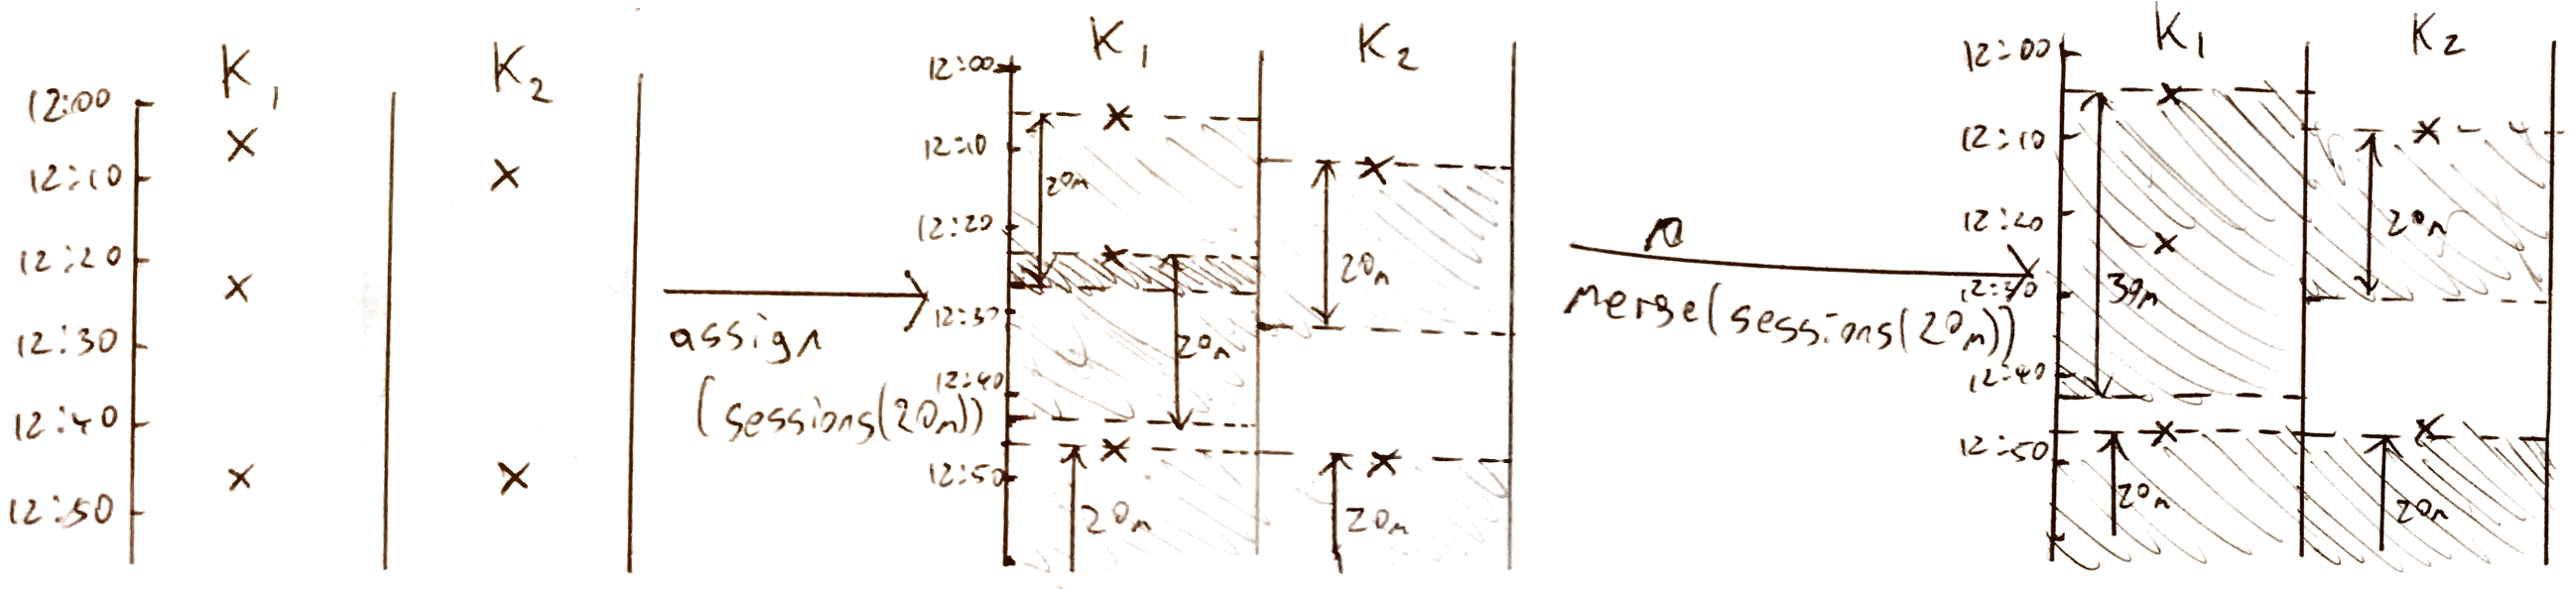
\includegraphics[width=\textwidth]{images/temp/sessions-assign-merge}
	\caption{The sessions windowing functions is used to assign elements with two separate keys into session-based windows. The \texttt{assign} operation puts each element in each key into its own 20 minute-long window. The \texttt{merge} operation then takes any overlapping windows and merges them into a larger window spanning all original windows.}
	\label{fig:prep:sessions-merge}
\end{figure}


\subsection{``The When'': Watermarks and triggers}\label{sec:prep:dataflow:when}

In the previous section, we have defined a way to group elements together into windows.
We have also asserted that we can ``emit a particular chunk of elements when we know that we have all the data for it''.
How can we achieve this in light of the fact that data may appear out of order?

The true answer is that we cannot---if we allow the possibility of unpredictably late data in our pipeline, then we cannot ever truly be certain that we can emit a complete pane of data.
What we can do, however, is introduce a model which allows us to specify the desired behaviour in a useful and flexible manner.
Let us first define the concept of \emph{watermarks}.

\subsubsection{Watermarks}

A \emph{watermark} is a lower bound, in event time, on the timestamps of values which have been processed by the pipeline (or a particular transform therein).
For example, if at a particular instant the watermark is time $T$, then we are promised that all events with timestamps earlier than $T$ have been processed.
A graph of watermark progression against processing time (such as the one in \cref{fig:prep:watermark-progression}) is a useful way to visualise the progress of a pipeline.
Further, this concept allows us to construct a powerful model of lateness in the system.
This is explored further in \cref{sec:impl:dataflow:lateness}.

\begin{figure}[h]
	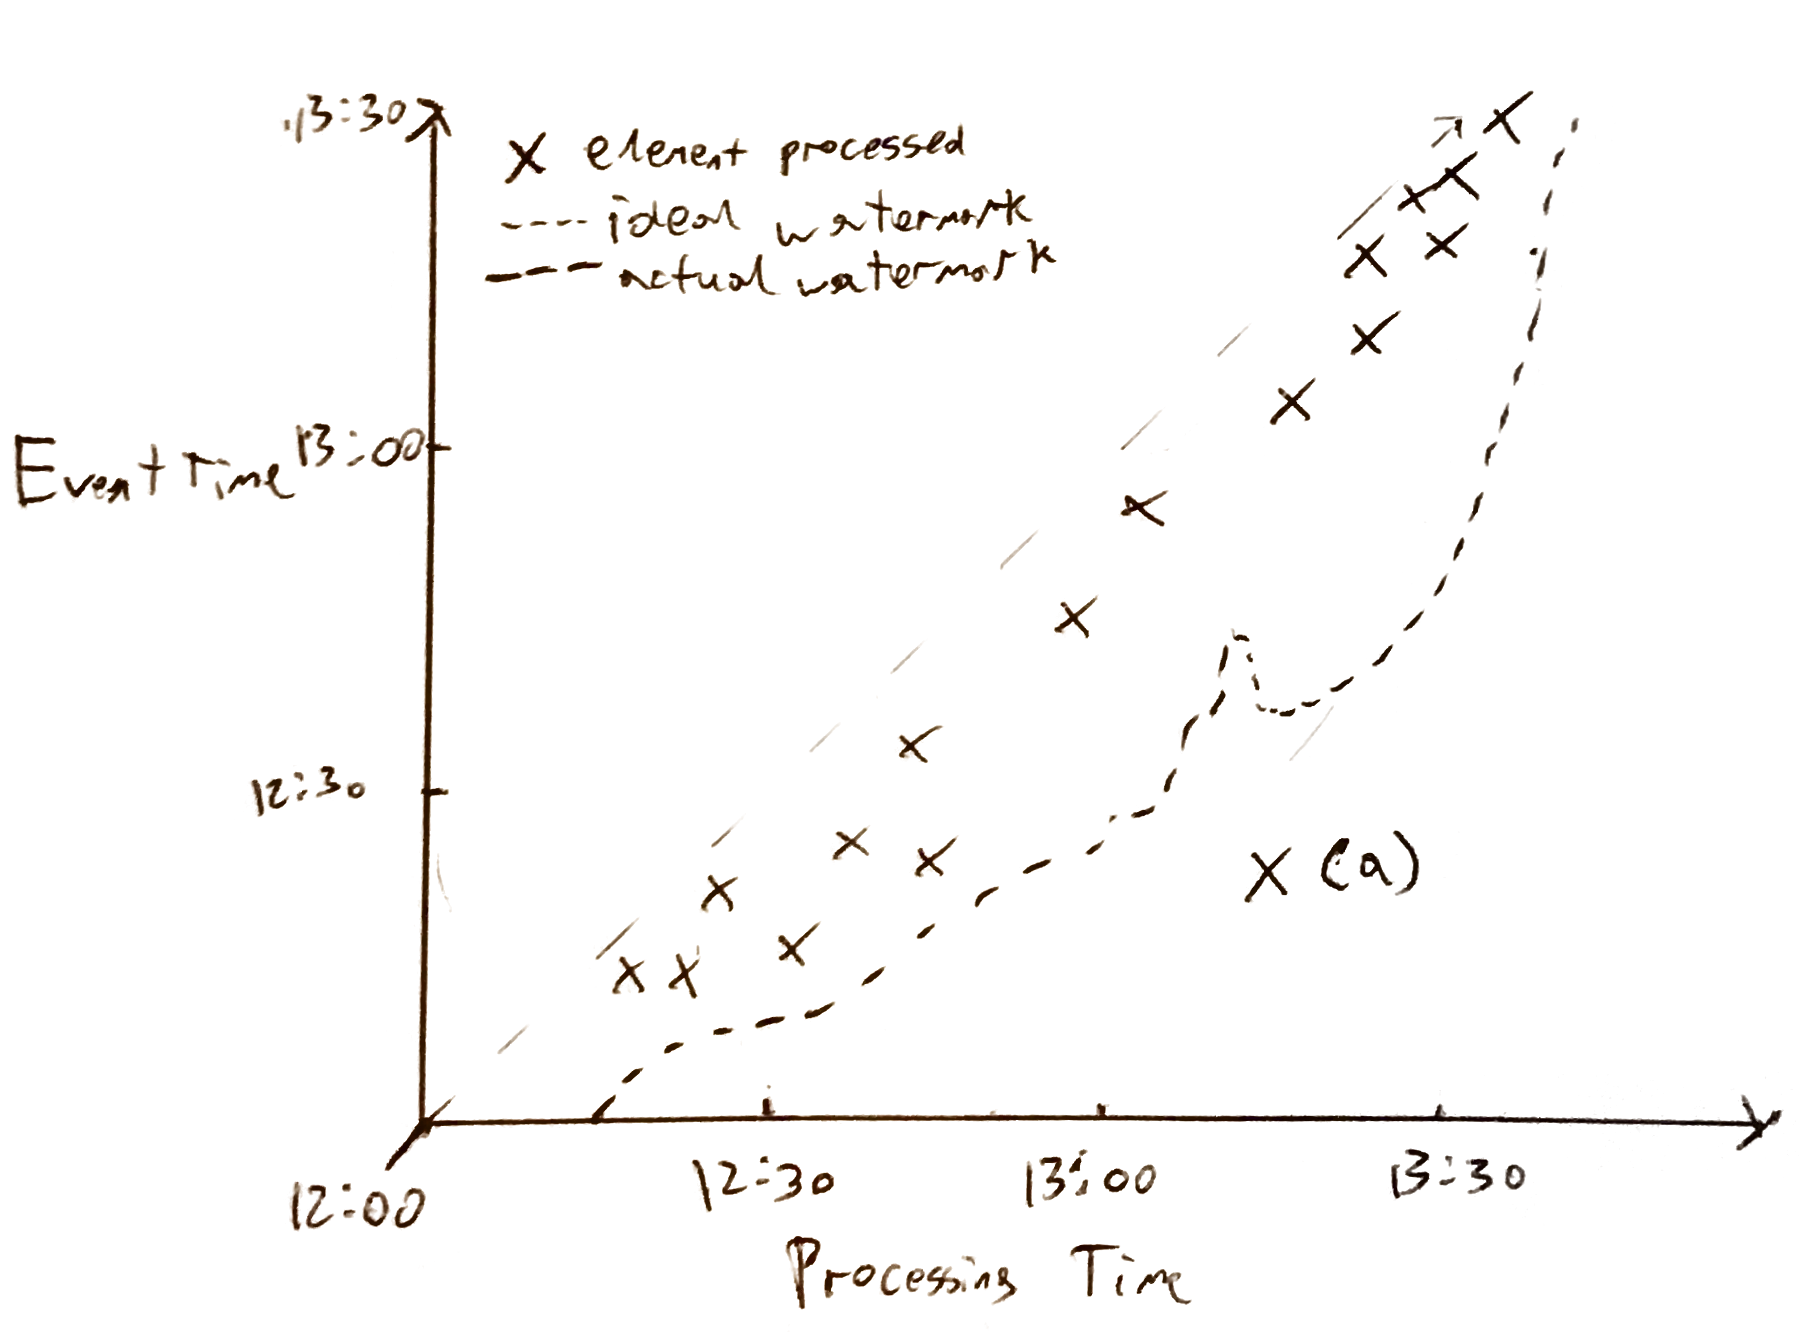
\includegraphics[width=\textwidth]{images/temp/watermark-progression-example}
	\caption{An example of a watermark progression. The ideal watermark shows the best possible result---processing each element immediately as it is produced. The actual watermark is a heuristic for the actual watermark for the system. We can see that the element marked (a) arrived behind the watermark---it was unexpectedly late to arrive and will be in fact marked as late.}
	\label{fig:prep:watermark-progression}
\end{figure}

The reader may at this point be asking, ``where does the watermark come from?''
Watermarks in the Dataflow Model are heuristics generated by sources of data, or by user logic in the pipeline.
Their exact behaviour is described in \cref{sec:impl:todo}.

\subsubsection{Triggering model}

An initial suggestion may be to simply use the watermark as an indication of when a window is finished and is safe to emit; that is, to emit once the watermark has passed the end of the window.
There are two major shortcomings with this strategy:
\begin{itemize}
	\item The watermark may be \textbf{too fast}---we may have decided that all elements for a given window have been seen and emit a pane, only to later on receive a late element which should have been in the window.
	It is unclear what to do with the element in this case.
	
	\item The watermark may be \textbf{too slow}---the heuristic can be too conservative, and even when we have access to the true watermark and not merely a heuristic, a single slow datum can hold up processing for the entire pipeline.
	Therefore using watermarks as the sole signal for emitting data can lead to high latency which may be highly undesirable in some scenarios.
\end{itemize} 

To solve these problems, we define a more complex triggering model.

Firstly, we explicitly allow for data in a particular window to be emitted multiple times.
We call each such emission a pane, and every pane is marked as either early, on-time or late.
Secondly, we define a trigger as simply some arbitrary code which has access to time information of elements passing through the transform, as well as watermark and other timing information.
In practice, we define a tree of triggers allowing us to easily achieve desired results (this is explored further in <todo ref>). 

In this manner we can allow for many different behaviours---for example, we may want to receive approximate results (early panes) every ten seconds (in processing time) until the watermark passes the end of the window, at which point an on-time pane is emitted.
Any further late data arriving after the watermark can trigger the emission of a late pane.
This, and myriad other combinations, are all possible with this model.
A key strength is that it decouples the marking of data as early/tentative, on-time/definitive, or late/corrective, from processing the different panes in different ways.

\todo{maybe include a description of a particular use case and which options one would choose for it?}

The combination of these flexible windowing and triggering models allow for a powerful, yet predictable method of grouping and emitting data as needed, even if it is sourced from a mixture of heterogeneous, unordered, infinite streams.
To provide these advantages, however, a surprising amount of extra machinery is required.
This is described in more detail in \cref{sec:impl:dataflow}.

\subsection{``The How'': Refinements and retractions}\label{sec:prep:dataflow:how}

While the concepts defined so far allow us to specify when panes should be emitted, we have not yet settled on what their contents should be, exactly.
We do this by selecting from one of the three refinement modes for a particular \verb|GroupByKey| transform:
\begin{itemize}
	\item The \textbf{discarding} mode simply discards the contents of the window after emitting a pane, such that any new pane emitted will contain only data received since the last emission. There is no relation between the contents of any two panes.
	\item The \textbf{accumulating} mode retains the contents of the window after emitting a pane. A later pane will include all of the data from the initial pane, in addition to any data which has arrived since.
	\item The \textbf{accumulating \& retracting} mode emits retractions to previous panes emitted, as well as following the semantics of the accumulating mode. This means that downstream transforms will first receive notification that the previous pane is now invalid (along with the contents of that pane again, to aid in undoing its results), and after this they will receive the contents of the new pane (which includes the contents of the initial pane, now refined with additional data). 
\end{itemize}

\todo{example of when to use one or the other?}

While the Model broadly defines the concept of retractions and how they may work at a high level, their implementation remains an unsolved problem and is actively worked on by the Beam project.
The main difficulty lies in the explosion of cached state which seems to be needed in order to allow the undoing of certain operations.
Therefore, the implementation and precise specification of the behaviour of retractions are out of the scope of this dissertation, and will not be mentioned again.

\section{Changing goals}

A side-effect of the way the Dataflow/Beam project has developed is that a large amount of development of the theory of the Model has occurred implicitly while the software was worked on.
New concepts were added \emph{in situ}, without an abstract definition.
Rather, informal proposals were written and iterated upon in code.

Therefore, a huge part of this project was the extraction and reverse-engineering of these concepts from the Java codebase into a more approachable specification.
This was further necessitated by the move from OOP to a functional approach, requiring each concept to be reduced to what it is in the abstract rather than just transferring the class hierarchy to a new language.

The initial project goals did not account for this---it was assumed that a reasonable implementation could be produced from the Dataflow paper \cite{Akidau:2015} using the Beam code simply as reference.
This interleaving of research and engineering required a particular approach to the execution of the project in order to prove successful.


\section{Software Engineering methods}\label{sec:prep:softeng}

\subsection{The spiral model}

The highly fluid goals of the project resulted in a need for a highly adaptive and agile development process, since fundamental assumptions made initially changed many times over.
Often core modules had to be re\"implemented multiple times over, as the model being extracted from the existing codebase grew more complete.

The Elixir language, with its clear modular structure combined with writing simple, composable functions enabled a flexible model where key logic in the codebase could be refactored with ease when needed.
While its explicit nature meant that modules did have to be rewritten instead of functionality piled on top as would be possible in a mutable OOP language, this in fact resulted in cleaner and more maintainable code with a clear focus.

Owing to this, a spiral model <ref?> of development was adopted, with core modules prototyped, integrated, and then refactored, extended or rewritten as other parts of the system demanded it.
The process is illustrated in \cref{fig:prep:spiral-model}.
Overall three or four iterations of prototyping and evaluating were performed, going all the way from a basic proof-of-concept to a working system implementing most key features of the Model.

\begin{figure}[h]
	\centering
	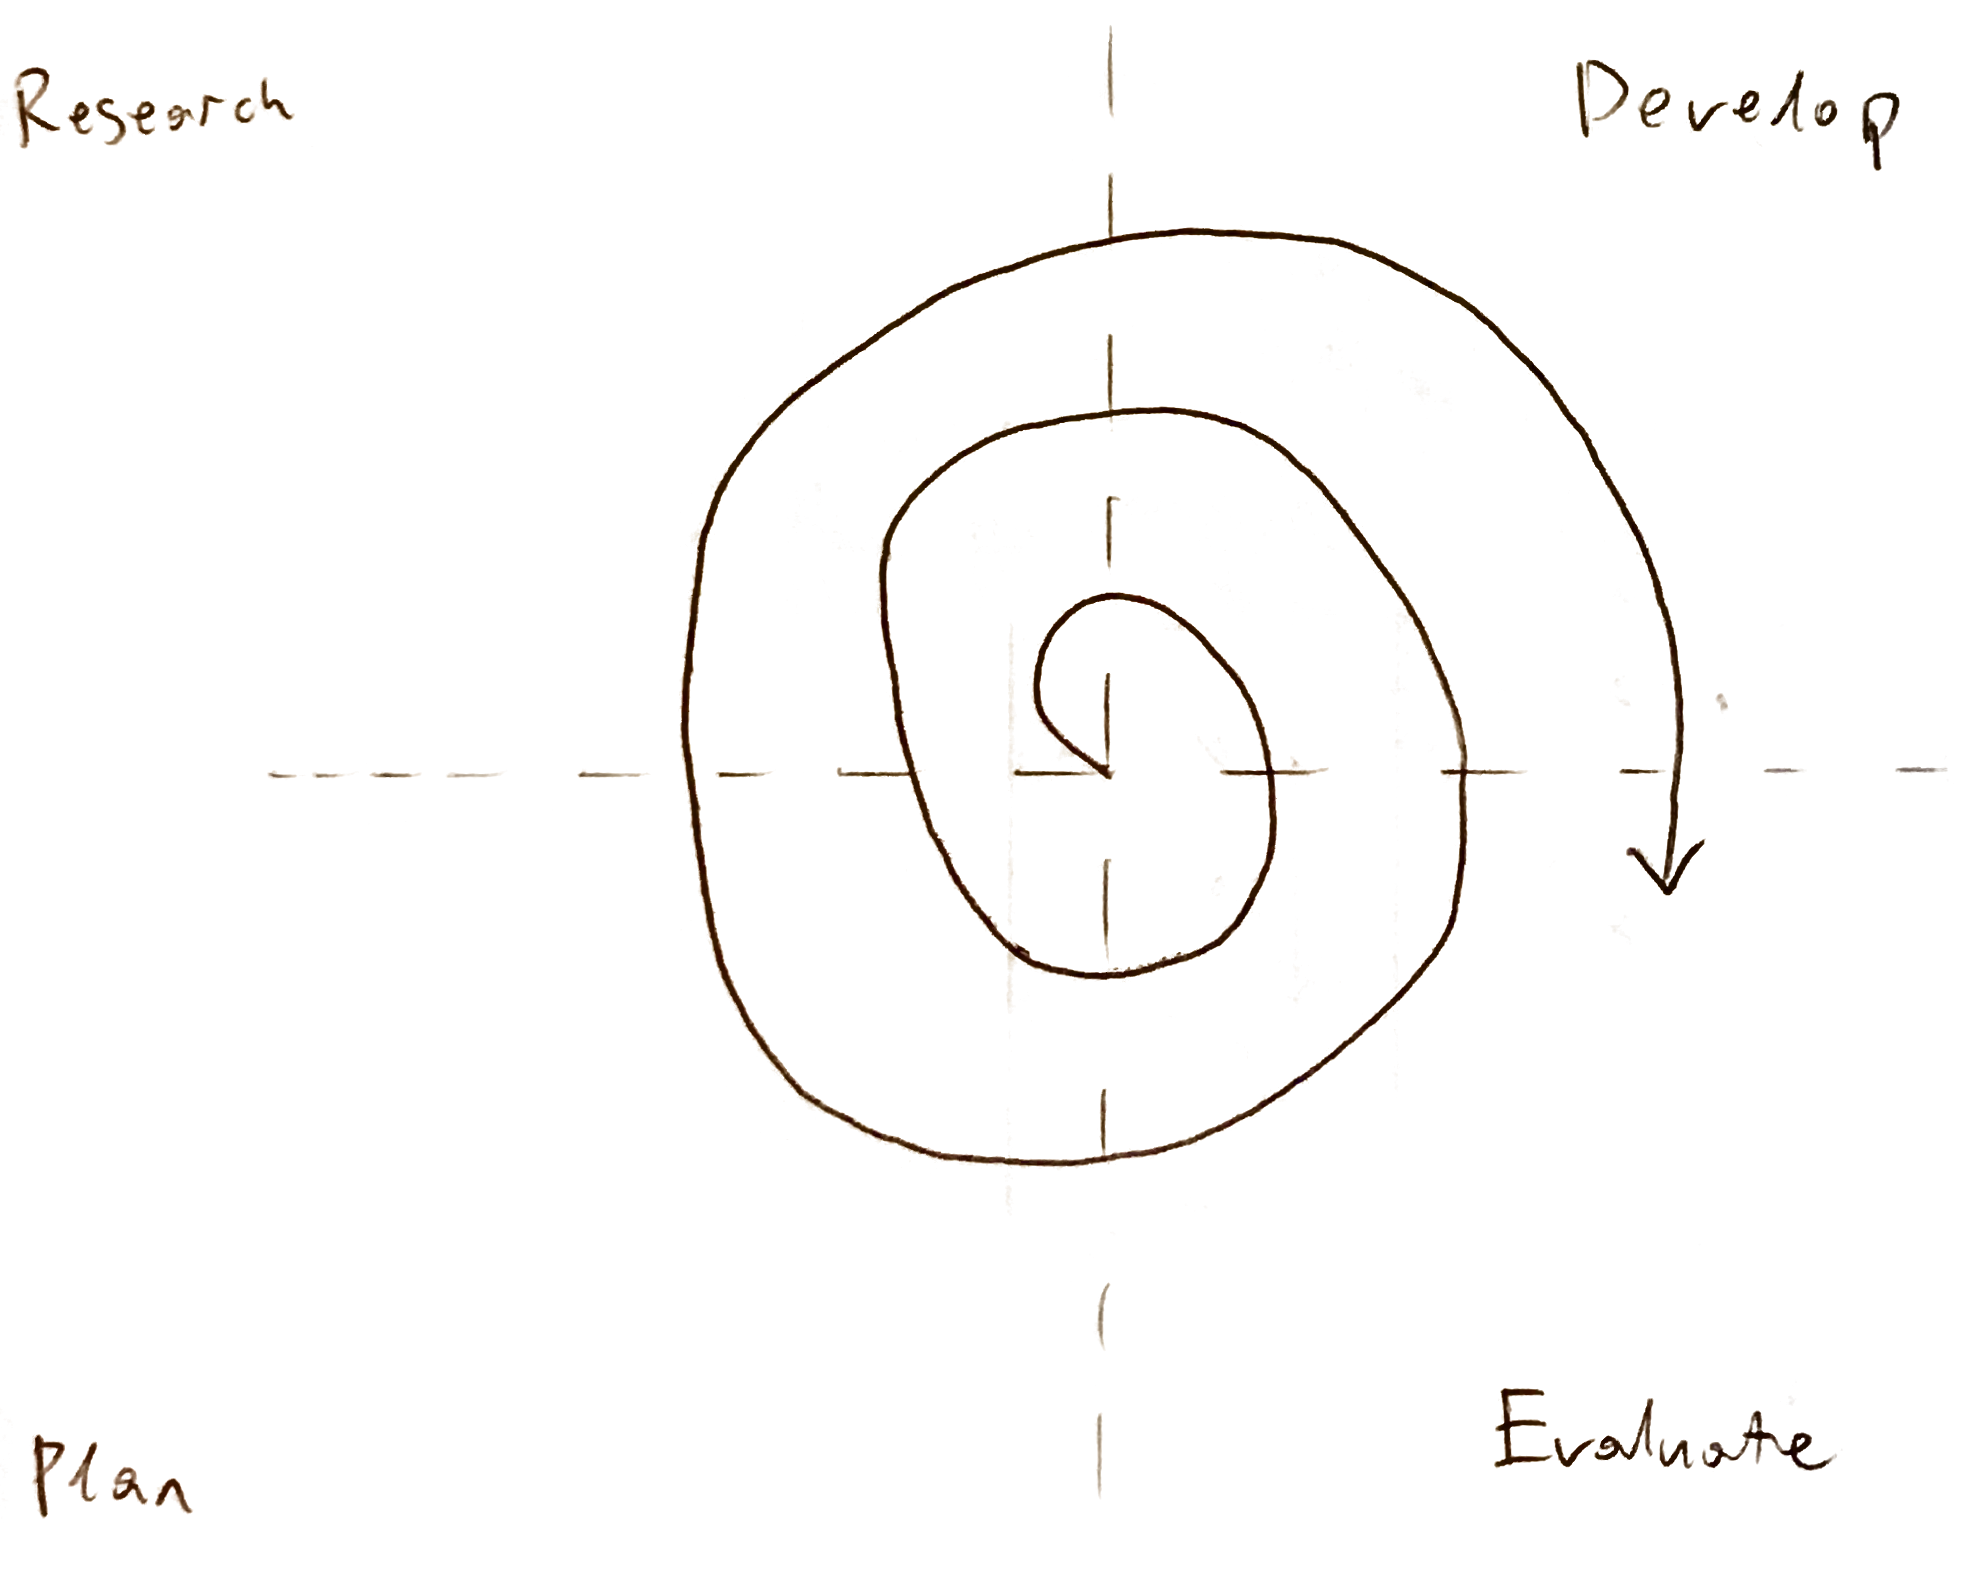
\includegraphics[width=0.6\textwidth]{images/temp/spiral}
	\caption{The spiral model of development as used in this project.}
	\label{fig:prep:spiral-model}
\end{figure}


\todo{Flesh the diagram out more, maybe indicate the features completed at each prototype iteration?}

\subsection{Source code management}

The project source code was maintained using Git, including a private GitHub upstream repository.
Source control was used to checkpoint and document progress.

It was especially important with the speculative nature of much code, making it easy and safe to ``move fast and break things''.

The dissertation sources were also kept in Git, with all project data being synced to Dropbox as well as an external backup service to guard against data loss.

\subsection{Testing approach}

Owing to the modular nature of Elixir making it easy to write small modules with pure functions, module-level testing was employed.
Small tests were written in order to check the invariants required by the model were satisfied by the implementation.

\todo{No they weren't. Either write the tests or take this out.}

Additionally, several end-to-end examples were written to exercise the entire system.
Some of these were also re\"implemented in Java and used for comparison purposes in the evaluation phase of the project.

\section{Starting point}\label{sec:prep:starting}

The project was started ``from scratch''---all core code in the implementation was written specifically for this project, during the timeframe of the project itself.
The author had a good working knowledge of Elixir, having had implemented several project in it before, but had no experience in working with Dataflow or Beam.

The Beam project was open-source and was used as a reference, but as explained, due to fundamental paradigm differences the project did not simply consist of transferring the OOP hierarchy of the system from one language to another.

\section{Summary}\label{sec:prep:summary}

\todo{is this needed?}